
\addtocontents{toc}{\vspace{\baselineskip}APPENDICES}
\setcounter{table}{0}
\renewcommand{\thetable}{\Alph{chapter}\arabic{table}}
\GrizzAppendix{Tables and Figures} \label{ch:extra}

\begin{sidewaystable}
\caption{Geographic information of sampling points at each  surveyed lakes }
\label{tab:Surveyed Lakes}
\begin{center}
\scalebox{0.86}{
\begin{tabular}{lllrrl}
\hline \\
\multicolumn{1}{c}{Name of Lake} & \multicolumn{1}{c}{Shorten Code} & \multicolumn{1}{c}{County} & \multicolumn{1}{c}{Longitude} & \multicolumn{1}{c}{Latitude} &
\multicolumn{1}{c}{HUC 14 Reachcode} \\ \hline
Bear Lake & BEA & Kalkaska & -84.9438079727 & 44.7286139551 & 04060103001048 \\
Belleville Lake & BEL & Wayne & -83.4663770506 & 42.2145253455 & 04090005001822 \\
Bogie Lake & BOG & Oakland & -83.5054334514 & 42.6188513679 & 04090005001348 \\
Brighton Lake & BRI & Livingston & -83.7958137995 & 42.5169054061 & 04090005001500 \\
Coldwater Lake & COL & Isabella & -84.9565922285 & 43.6613607551 & 04080202000902 \\
Deer Lake & DEE & Charlevoix & -84.9770123186 & 45.166441811 & 04060105001116 \\
Ford Lake & FOR & Washtenaw & -83.5849122567 & 42.2159133043 & 04090005001823 \\
Houghton Lake & HOU & Roscommon & -84.7262816343 & 44.3385407778 & 04060102002461 \\
Hudson Lake & HUD & Lenawee & -84.2545514803 & 41.835000535 & 04100002001317 \\
Intermediate lake & INT & Antrim & -85.2293359783 & 45.0265435299 & 04060105003435 \\
Lake Cadillac & CAD & Wexford & -85.4266252378 & 44.2410192547 & 04060102001951 \\
Lake Margrethe & MAR & Crawford & -84.7830175986 & 44.6464747348 & 04060103001058 \\
Lake Nepessing & NEP & Lapeer & -83.3728265865 & 43.0161554865 & 04080204001601 \\
Lime Lake & LIM & Hillsdale & -84.3791188315 & 41.7861576065 & 04100006000872 \\
Little Glen Lake & LGL & Leelanac & -85.963633169 & 44.8687577197 & 04060104000456 \\
Little Round Lake & LRO & Lenawee & -84.3527742524 & 41.9093334799 & 04100006000858 \\
Manitou Lake & MAN & Shiawassee & -84.2038069227 & 42.925537136 & 04050005000939 \\
Ore Lake & ORE & Livingston & -83.7959940227 & 42.4805569493 & 04090005001574 \\
Paradise Lake & PAR & Emmett & -84.7512093045 & 45.6872890124 & 04060105001063 \\
Platte Lake & PLA & Benzie & -86.092789204 & 44.6900468421 & 04060104000558 \\
Pontiac Lake & PON & Oakland & -83.451096479 & 42.6664394508 & 04090005001288 \\
Posey lake & POS & Lenawee & -84.3007962072 & 41.8970465491 & 04100006000857 \\
Round Lake & ROU & Lenawee & -84.1318219224 & 42.0712488438 & 04100002001130 \\
Sanford Lake & SAN & Midland & -84.3860517762 & 43.7104273774 & 04080201001468 \\
Silver Lake & SIL & Grand Traverse & -85.687150728 & 44.6980286859 & 04060105003542 \\
Stony Creek Lake & STO & Oakland & -83.0870627175 & 42.7260717429 & 04090003001029 \\
Sugden Lake & SUG & Oakland & -83.4972563639 & 42.6173106359 & 04090005001347 \\
West Twin Lake & WTL & Montmorency & -84.3501403918 & 44.8762035424 & 04070007001271 \\
Wixom Lake & WIX & Gladwin & -84.3537506311 & 43.8276751177 & 04080201001442 \\ \hline
\multicolumn{3}{r}{{HUC=Hydrological Unit Code}} \\ \hline
\multicolumn{3}{r}{{GPS Coordinates are in decimal degrees, North American Datum of 1983 (NAD83)}} \\ \hline
\end{tabular}}
\end{center}
\end{sidewaystable}





\begin{figure}[!ht]
\scalebox{1.14}{
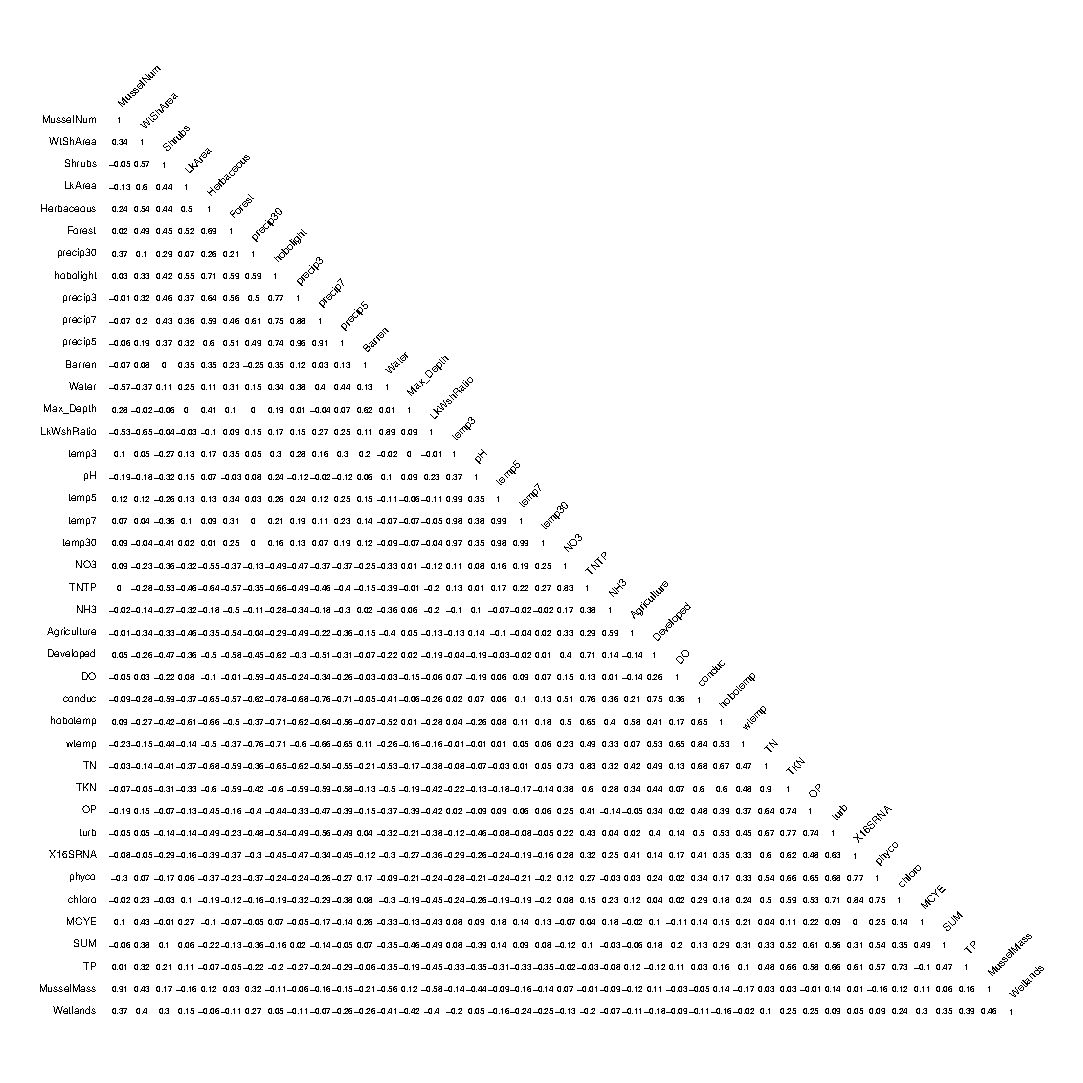
\includegraphics[width=\textwidth]{figures/matrixfull}}
\caption{Correlation matrix displaying Pearson's coefficient on the full data.}
\label{fig:matrixfull}
\end{figure}








\begin{table}[!ht]
\centering
  \caption{Microcystin congener statistical summary}
  \label{}
\begin{tabular}{@{\extracolsep{5pt}}lccccc}
\\[-1.8ex]\hline
\hline \\[-1.8ex]
Statistic & \multicolumn{1}{c}{N} & \multicolumn{1}{c}{Mean} & \multicolumn{1}{c}{St. Dev.} & \multicolumn{1}{c}{Min} & \multicolumn{1}{c}{Max} \\
\hline \\[-1.8ex]
Nodularin & 114 & 0.0003 & 0.002 & ND & 0.021 \\
{[D-Asp3]}MC-RR & 114 & 0.006 & 0.028 & ND & 0.255 \\
MC-RR & 114 & 0.185 & 0.855 & ND & 8.552 \\
MC-YR & 114 & 0.046 & 0.202 & ND & 1.799 \\
MC-HtyR & 114 & 0.002 & 0.012 & ND & 0.107 \\
MC-LR & 114 & 0.142 & 0.447 & ND & 3.570 \\
{[D-Asp3]}MC-LR & 114 & 0.027 & 0.107 & ND & 0.902 \\
MC-HilR & 114 & 0.004 & 0.019 & ND & 0.150 \\
MC-WR & 114 & 0.005 & 0.029 & ND & 0.302 \\
MC-LA & 114 & 0.088 & 0.196 & ND & 1.729 \\
MC-LY & 114 & 0.0004 & 0.002 & ND & 0.024 \\
MC-LW & 114 & ND & ND & ND & ND \\
MC-LF & 114 & 0.0002 & 0.001 & ND & 0.012 \\
MC Sum from LC MS/MS  & 114 & 0.505 & 1.580 & ND & 14.857 \\
MC from ELISA & 115 & 0.747 & 1.784 & ND & 15.320 \\
\hline \\[-1.8ex]
\multicolumn{6}{r}{Values are expressed as($\mu$g of MC*${L^{-1}}$)} \\
\multicolumn{6}{r}{ND=No Detects} \\
\end{tabular}
\end{table}

%congnenr plot by latitiude
\begin{figure}[!ht]
  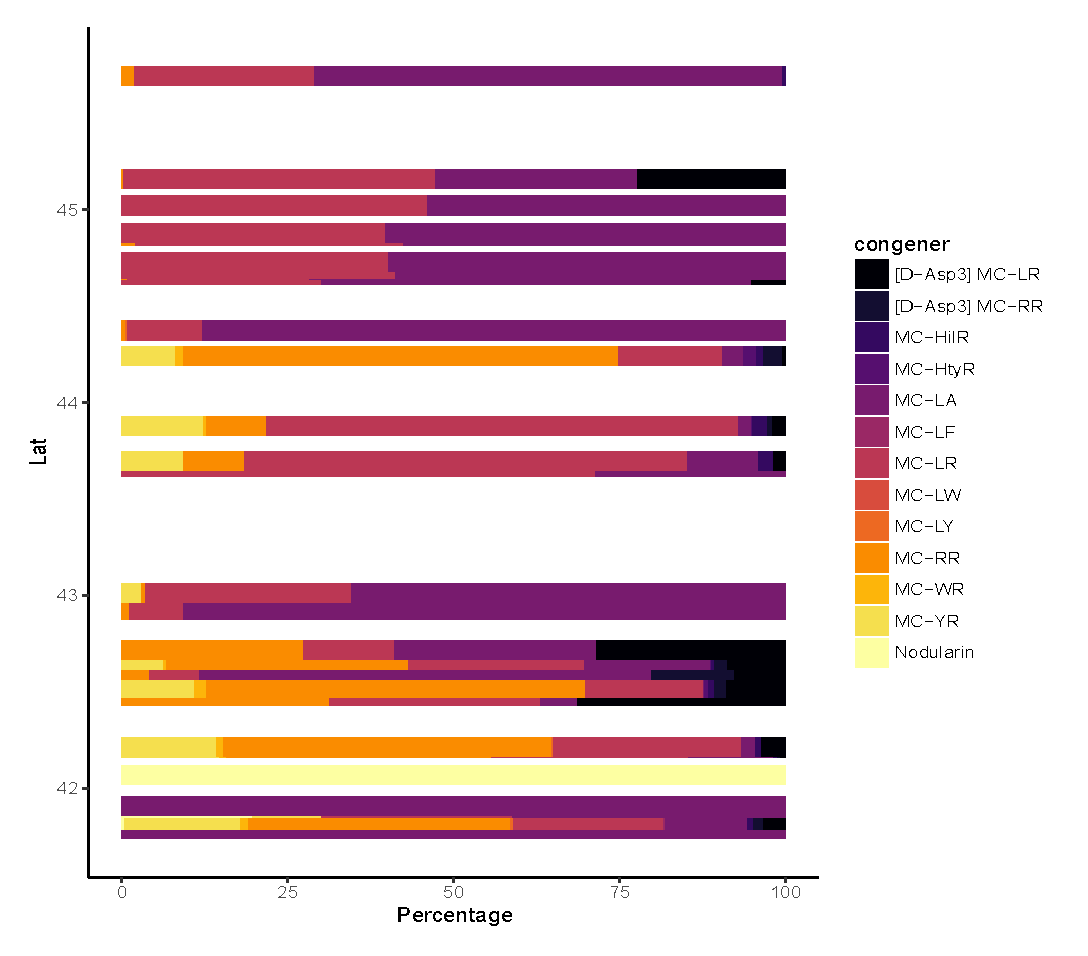
\includegraphics[width=\textwidth]{congeners}
    \caption{Proportion of MC congeners plotted by latitude}
  \label{congenerlat}
\end{figure}

\begin{table}[!ht]
  \centering
  \caption{QPCR statistical summary table}
  \label{QPCR}
  \begin{tabular}{@{\extracolsep{5pt}}lccccc}
  \\[-1.8ex]\hline
  \hline \\[-1.8ex]
  Statistic & \multicolumn{1}{c}{N} & \multicolumn{1}{c}{Mean} & \multicolumn{1}{c}{St. Dev.} & \multicolumn{1}{c}{Min} & \multicolumn{1}{c}{Max} \\
  \hline \\[-1.8ex]
  16S rRNA & 112 & 405,761 & 798,946 & ND & 6,765,631 \\
  mcyE & 91 & 8,517 & 49,396 & ND & 467,174 \\
  cyrA & 93 & ND & ND & ND & ND \\
  sxtA & 93 & ND & ND & ND & ND \\
  \hline \\[-1.8ex]
  \multicolumn{6}{r}{Values are expressed as Gene copies/mL} \\
  \multicolumn{6}{r}{ND=No Detects} \\
  \end{tabular}
  \end{table}

  \begin{figure}[!hp]
  \centering
    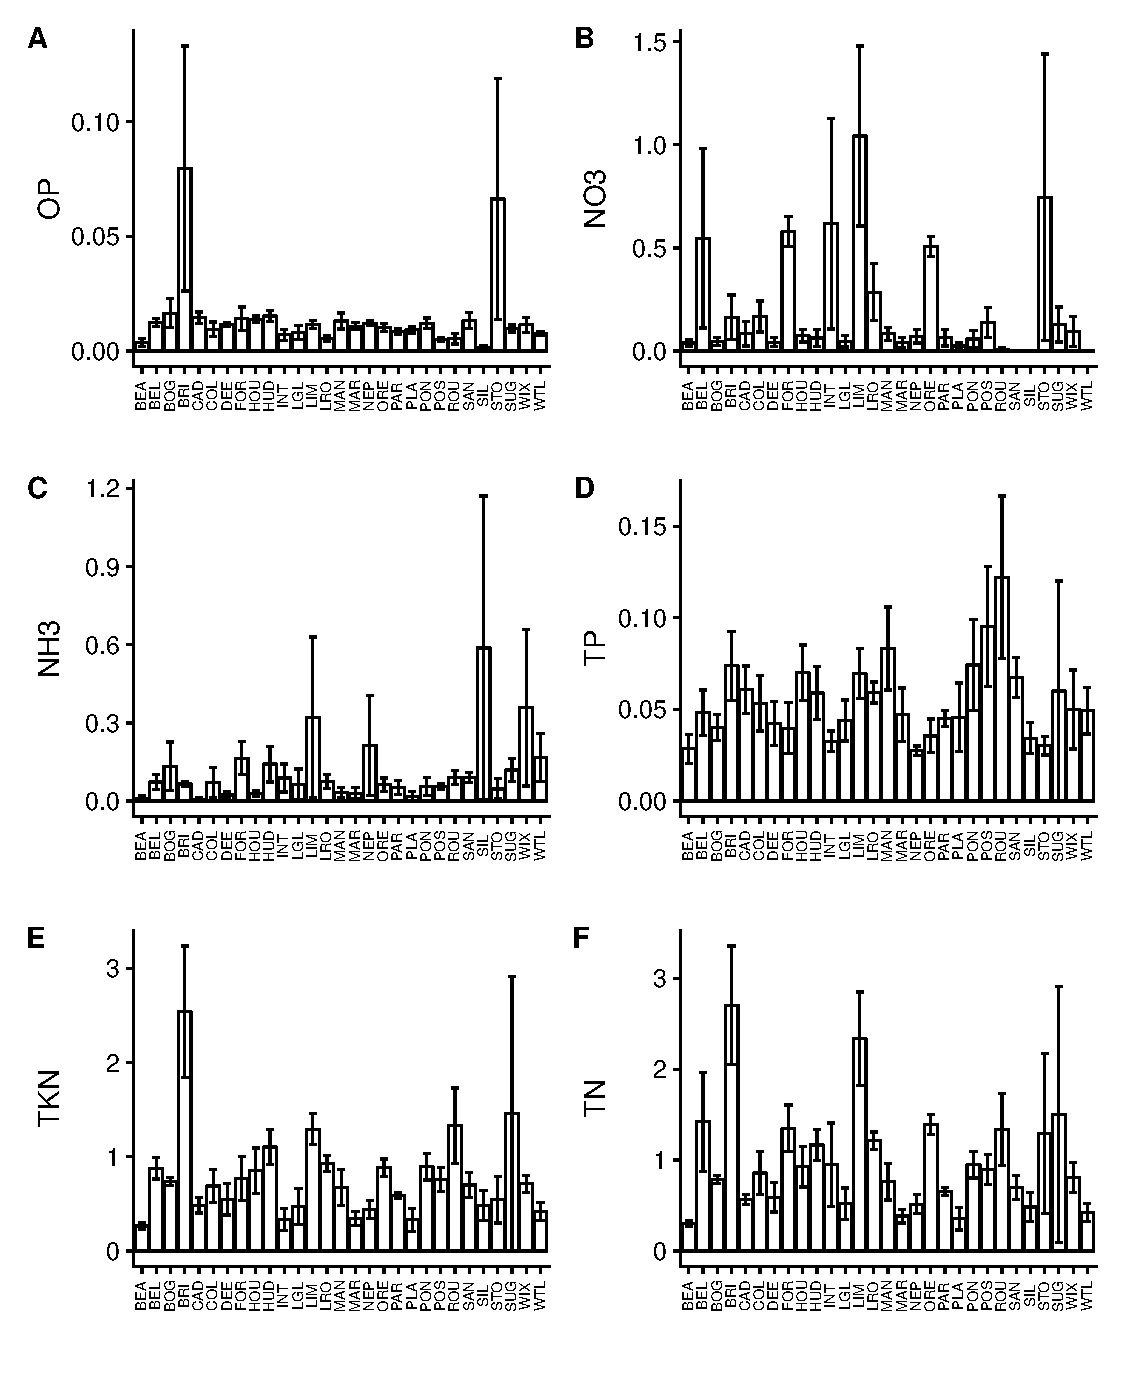
\includegraphics[width=\textwidth]{figures/nutboxplotlake}
    \caption{Average nutrient concentrations for each lake. Orthophosphate (mg-P/L) in figure (A), nitrate+nitrite (mg-N/L) in figure (B), ammonia (mg-N/L) in figure (C), total phosphorus (mg-P/L) in figure (D) and total Kjeldahl nitrogen (mg-N/L) in figure (E). Error bars represents one standard deviation of the mean. }
    \label{fig:nutrients}
  \end{figure}


  \begin{table}[!ht]
    \centering
    \caption{Lake nutrients statistical summary}
    \label{}
  \begin{tabular}{@{\extracolsep{5pt}}lccccc}
  \\[-1.8ex]\hline
  \hline \\[-1.8ex]
  Statistic & \multicolumn{1}{c}{N} & \multicolumn{1}{c}{Mean} & \multicolumn{1}{c}{St. Dev.} & \multicolumn{1}{c}{Min} & \multicolumn{1}{c}{Max} \\
  \hline \\[-1.8ex]
   Orthophosphate (mg P/L) & 114 & 0.015 & 0.030 & ND & 0.237 \\
  Nitrate+Nitrite (mg N/L) & 115 & 0.199 & 0.443 & ND & 2.827 \\
  Ammonia (mg N/L)  & 115 & 0.112 & 0.281 & ND & 2.338 \\
  Total Phosphorus (mg P/L) & 114 & 0.055 & 0.037 & ND & 0.239 \\
  Total Kjeldahl Nitrogen (mg N/L) & 114 & 0.763 & 0.602 & ND & 4.555 \\
  Total Nitrogen & 114 & 1.074 & 0.870 & 0.103 & 4.717 \\
  \hline \\[-1.8ex]
  \multicolumn{6}{r}{ND=No Detects} \\
  \end{tabular}
  \end{table}

  \begin{figure}[!hp]
  \centering
    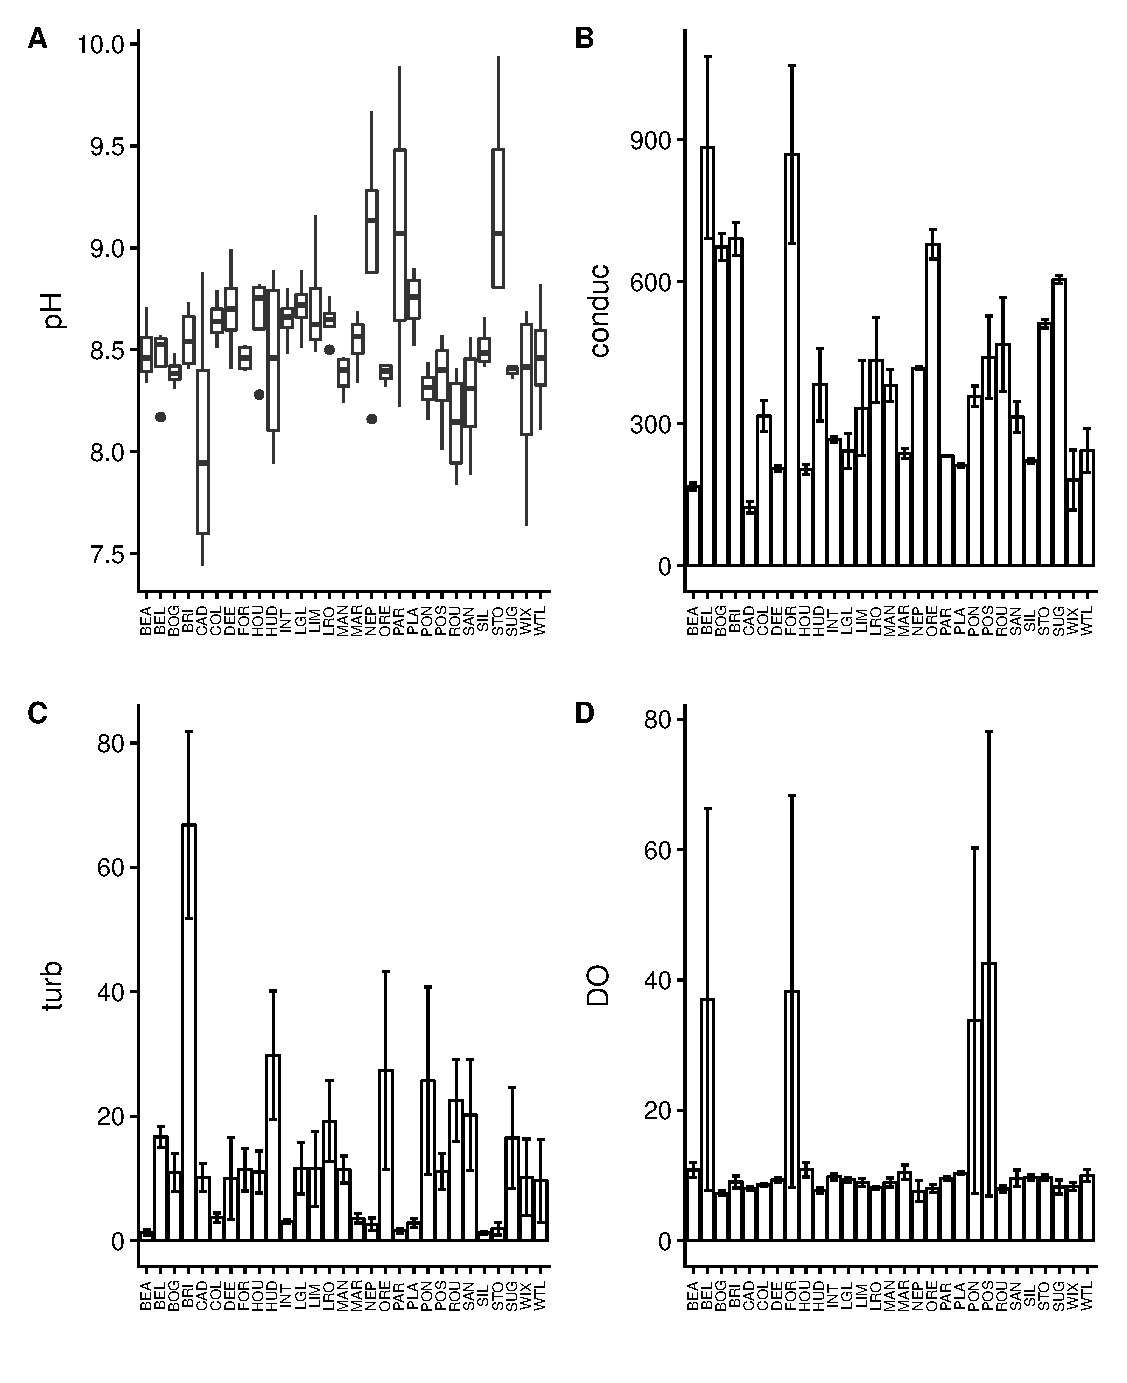
\includegraphics[width=\textwidth]{figures/watboxplotlake.eps}
    \caption{Summary of measured water chemical parameters: A box and whisker plot of pH in figure (A). Bar plots of average conductance (B), average turbidity (C), and average dissolved oxygen (D) plotted by each lake. }
  \end{figure}
